\subsection{三阶行列式}\label{subsec:4-2}

把九个数排成三行三列,在这九个数的两旁各加一条竖线,如
\begin{equation}
    \begin{vmatrix}
        a_1 & b_1 & c_1 \\
        a_2 & b_2 & c_2 \\
        a_3 & b_3 & c_3
    \end{vmatrix}, \label{eq:sjhls-1}
\end{equation}
并且规定它表示
\begin{equation}
    a_1b_2c_3 + a_2b_3c_1 + a_3b_1c_2 - a_3b_2c_1 - a_2b_1c_3 - a_1b_3c_2 \text{。} \label{eq:sjhls-2}
\end{equation}
这时,\eqref{eq:sjhls-1} 式叫做 \textbf{三阶行列式}。三阶行列式有三行三列。

三阶行列式也可按对角线法则展开。如图:

\begin{figure}[H]
    \centering
    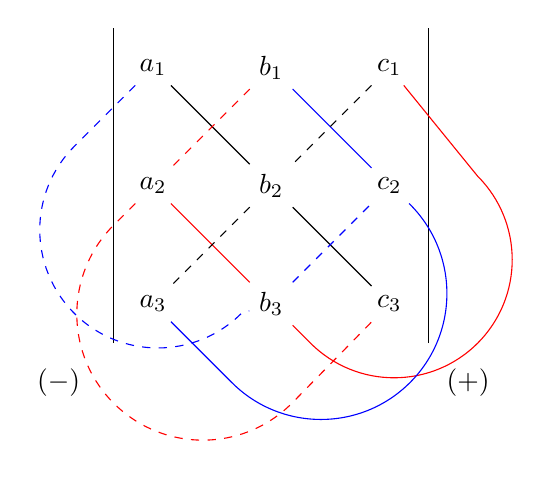
\begin{tikzpicture}
    \draw (-0.5, -0.5) -- (-0.5, 3.5);
    \draw (3.5, -0.5) -- (3.5, 3.5);
    \foreach \x/\y/\txt/\name in {
        0/0/a_3/a3,   0/1.5/a_2/a2,   0/3/a_1/a1,
        1.5/0/b_3/b3, 1.5/1.5/b_2/b2, 1.5/3/b_1/b1,
        3/0/c_3/c3,   3/1.5/c_2/c2,   3/3/c_1/c1,
     } {
        \node (\name) at (\x, \y) {$\txt$};
    }
    \draw (a1) -- (b2) -- (c3);
    \draw [red] (a2) -- (b3) -- +(0.5, -0.5) arc (225:405:1.5) -- (c1);
    \draw [blue] (a3) -- +(1, -1) arc(225:405:1.6) -- (c2) -- (b1);

    \draw [dashed, blue] (a1) -- +(-1, -1) arc(135:315:1.5) -- (b3) -- (c2);
    \draw [dashed, red] (b1) -- (a2) -- +(-0.5, -0.5) arc(135:315:1.6) -- (c3);
    \draw [dashed] (c1) -- (b2) -- (a3);

    \node at (-1.2, -1) {$(-)$};
    \node at (4, -1) {$(+)$};
\end{tikzpicture}

\end{figure}


图中实线上三个元素的积,添上正号;虚线上三个元素的积,添上负号。容易看出三阶行列式就是这六项的和。

\liti 用对角线法则计算行列式
$$\begin{vmatrix*}[r]
    3  & -2 & 1 \\
    -2 & 1  & 3 \\
    2  & 0  & -2
\end{vmatrix*} \text{。} $$

\jie $\begin{aligned}[t]
    & \begin{vmatrix*}[r]
        3  & -2 & 1 \\
        -2 & 1  & 3 \\
        2  & 0  & -2
    \end{vmatrix*} \\
    ={} & 3 \times 1 \times (-2) + (-2) \times 0 \times 1 + 2 \times (-2) \times 3 \\
        & -2 \times 1 \times 1 - (-2) \times (-2) \times (-2) - 3 \times 0 \times 3 \\
    ={} & -6 + 0 -12 - 2 + 8 - 0 = -12 \text{。}
\end{aligned}$


\lianxi
\begin{xiaotis}

\xiaoti{用对角线法则计算:}
\begin{xiaoxiaotis}

    \renewcommand\arraystretch{1.2}
    \begin{tabular}[t]{*{2}{@{}p{16em}}}
        \xiaoxiaoti{
            $\begin{vmatrix*}[r]
                1 & 5 & 7 \\
                2 & 0 & -4 \\
                -3 & 1 & 6
            \end{vmatrix*}$;
        } & \xiaoxiaoti{
            $\begin{vmatrix*}[r]
                2 & -3 & 1 \\
                4 & -1 & 7 \\
                -1 & 5 & 2
            \end{vmatrix*}$。
        }
    \end{tabular}

\end{xiaoxiaotis}



\xiaoti{用对角线法则展开下列行列式,并化简:}
\begin{xiaoxiaotis}

    \renewcommand\arraystretch{1.2}
    \begin{tabular}[t]{*{2}{@{}p{16em}}}
        \xiaoxiaoti{
            $\begin{vmatrix}
                0 & a & b \\
                a & 0 & c \\
                b & c & 0
            \end{vmatrix}$;
        } & \xiaoxiaoti{
            $\begin{vmatrix}
                x & y & z \\
                z & x & y \\
                y & z & x
            \end{vmatrix}$;
        }\\

        \xiaoxiaoti{
            $\begin{vmatrix*}[r]
                a & b & c \\
                2a & 2b & 2c \\
                m & n & l
            \end{vmatrix*}$;
        } & \xiaoxiaoti{
            $\begin{vmatrix*}[r]
                1 & -a & -b \\
                a & 1 & -c \\
                b & c & 1
            \end{vmatrix*}$。
        }
    \end{tabular}

\end{xiaoxiaotis}



\xiaoti{计算下列各题中的两个行列式;比较计算结果,得出每两个行列式之间的关系式。}
\begin{xiaoxiaotis}

    \xiaoxiaoti{
        $\begin{vmatrix}
            1 & 2 & 3 \\
            4 & 5 & 6 \\
            7 & 8 & 9
        \end{vmatrix}$,
        $\begin{vmatrix}
            1 & 4 & 7 \\
            2 & 5 & 8 \\
            3 & 6 & 9
        \end{vmatrix}$;
    }

    \xiaoxiaoti{
        $\begin{vmatrix*}[r]
            3 & 0 & 4 \\
            1 & 1 & 2 \\
            5 & -7 & 11
        \end{vmatrix*}$,
        $\begin{vmatrix*}[r]
            3 & 0 & 4 \\
            k & k & 2k \\
            5 & -7 & 11
        \end{vmatrix*}$。
    }

\end{xiaoxiaotis}

\end{xiaotis}
